% Options for packages loaded elsewhere
\PassOptionsToPackage{unicode}{hyperref}
\PassOptionsToPackage{hyphens}{url}
\PassOptionsToPackage{dvipsnames,svgnames*,x11names*}{xcolor}
%
\documentclass[
  11pt,
  krantz2, a4paper, twoside]{krantz}
\usepackage{amsmath,amssymb}
\usepackage{lmodern}
\usepackage{setspace}
\usepackage{ifxetex,ifluatex}
\ifnum 0\ifxetex 1\fi\ifluatex 1\fi=0 % if pdftex
  \usepackage[T1]{fontenc}
  \usepackage[utf8]{inputenc}
  \usepackage{textcomp} % provide euro and other symbols
\else % if luatex or xetex
  \usepackage{unicode-math}
  \defaultfontfeatures{Scale=MatchLowercase}
  \defaultfontfeatures[\rmfamily]{Ligatures=TeX,Scale=1}
  \setmainfont[]{NanumMyeongjo}
\fi
% Use upquote if available, for straight quotes in verbatim environments
\IfFileExists{upquote.sty}{\usepackage{upquote}}{}
\IfFileExists{microtype.sty}{% use microtype if available
  \usepackage[]{microtype}
  \UseMicrotypeSet[protrusion]{basicmath} % disable protrusion for tt fonts
}{}
\makeatletter
\@ifundefined{KOMAClassName}{% if non-KOMA class
  \IfFileExists{parskip.sty}{%
    \usepackage{parskip}
  }{% else
    \setlength{\parindent}{0pt}
    \setlength{\parskip}{6pt plus 2pt minus 1pt}}
}{% if KOMA class
  \KOMAoptions{parskip=half}}
\makeatother
\usepackage{xcolor}
\IfFileExists{xurl.sty}{\usepackage{xurl}}{} % add URL line breaks if available
\IfFileExists{bookmark.sty}{\usepackage{bookmark}}{\usepackage{hyperref}}
\hypersetup{
  pdftitle={신약개발을 위한 실전 약동학 (I - 이론과 자료해석)},
  pdfauthor={가톨릭대학교 계량약리학연구소(PIPET) 펴냄 (대표저자 임동석)},
  colorlinks=true,
  linkcolor=Maroon,
  filecolor=Maroon,
  citecolor=Blue,
  urlcolor=Blue,
  pdfcreator={LaTeX via pandoc}}
\urlstyle{same} % disable monospaced font for URLs
\usepackage{color}
\usepackage{fancyvrb}
\newcommand{\VerbBar}{|}
\newcommand{\VERB}{\Verb[commandchars=\\\{\}]}
\DefineVerbatimEnvironment{Highlighting}{Verbatim}{commandchars=\\\{\}}
% Add ',fontsize=\small' for more characters per line
\usepackage{framed}
\definecolor{shadecolor}{RGB}{248,248,248}
\newenvironment{Shaded}{\begin{snugshade}}{\end{snugshade}}
\newcommand{\AlertTok}[1]{\textcolor[rgb]{0.94,0.16,0.16}{#1}}
\newcommand{\AnnotationTok}[1]{\textcolor[rgb]{0.56,0.35,0.01}{\textbf{\textit{#1}}}}
\newcommand{\AttributeTok}[1]{\textcolor[rgb]{0.77,0.63,0.00}{#1}}
\newcommand{\BaseNTok}[1]{\textcolor[rgb]{0.00,0.00,0.81}{#1}}
\newcommand{\BuiltInTok}[1]{#1}
\newcommand{\CharTok}[1]{\textcolor[rgb]{0.31,0.60,0.02}{#1}}
\newcommand{\CommentTok}[1]{\textcolor[rgb]{0.56,0.35,0.01}{\textit{#1}}}
\newcommand{\CommentVarTok}[1]{\textcolor[rgb]{0.56,0.35,0.01}{\textbf{\textit{#1}}}}
\newcommand{\ConstantTok}[1]{\textcolor[rgb]{0.00,0.00,0.00}{#1}}
\newcommand{\ControlFlowTok}[1]{\textcolor[rgb]{0.13,0.29,0.53}{\textbf{#1}}}
\newcommand{\DataTypeTok}[1]{\textcolor[rgb]{0.13,0.29,0.53}{#1}}
\newcommand{\DecValTok}[1]{\textcolor[rgb]{0.00,0.00,0.81}{#1}}
\newcommand{\DocumentationTok}[1]{\textcolor[rgb]{0.56,0.35,0.01}{\textbf{\textit{#1}}}}
\newcommand{\ErrorTok}[1]{\textcolor[rgb]{0.64,0.00,0.00}{\textbf{#1}}}
\newcommand{\ExtensionTok}[1]{#1}
\newcommand{\FloatTok}[1]{\textcolor[rgb]{0.00,0.00,0.81}{#1}}
\newcommand{\FunctionTok}[1]{\textcolor[rgb]{0.00,0.00,0.00}{#1}}
\newcommand{\ImportTok}[1]{#1}
\newcommand{\InformationTok}[1]{\textcolor[rgb]{0.56,0.35,0.01}{\textbf{\textit{#1}}}}
\newcommand{\KeywordTok}[1]{\textcolor[rgb]{0.13,0.29,0.53}{\textbf{#1}}}
\newcommand{\NormalTok}[1]{#1}
\newcommand{\OperatorTok}[1]{\textcolor[rgb]{0.81,0.36,0.00}{\textbf{#1}}}
\newcommand{\OtherTok}[1]{\textcolor[rgb]{0.56,0.35,0.01}{#1}}
\newcommand{\PreprocessorTok}[1]{\textcolor[rgb]{0.56,0.35,0.01}{\textit{#1}}}
\newcommand{\RegionMarkerTok}[1]{#1}
\newcommand{\SpecialCharTok}[1]{\textcolor[rgb]{0.00,0.00,0.00}{#1}}
\newcommand{\SpecialStringTok}[1]{\textcolor[rgb]{0.31,0.60,0.02}{#1}}
\newcommand{\StringTok}[1]{\textcolor[rgb]{0.31,0.60,0.02}{#1}}
\newcommand{\VariableTok}[1]{\textcolor[rgb]{0.00,0.00,0.00}{#1}}
\newcommand{\VerbatimStringTok}[1]{\textcolor[rgb]{0.31,0.60,0.02}{#1}}
\newcommand{\WarningTok}[1]{\textcolor[rgb]{0.56,0.35,0.01}{\textbf{\textit{#1}}}}
\usepackage{longtable,booktabs,array}
\usepackage{calc} % for calculating minipage widths
% Correct order of tables after \paragraph or \subparagraph
\usepackage{etoolbox}
\makeatletter
\patchcmd\longtable{\par}{\if@noskipsec\mbox{}\fi\par}{}{}
\makeatother
% Allow footnotes in longtable head/foot
\IfFileExists{footnotehyper.sty}{\usepackage{footnotehyper}}{\usepackage{footnote}}
\makesavenoteenv{longtable}
\setlength{\emergencystretch}{3em} % prevent overfull lines
\providecommand{\tightlist}{%
  \setlength{\itemsep}{0pt}\setlength{\parskip}{0pt}}
\setcounter{secnumdepth}{5}
%\usepackage{tikz-cd} % \xleftrightarrow
%\usepackage{amsmath} 
%\documentclass[b5paper,9pt]{extarticle}
%\usepackage{geometry}

%\usepackage[%
%  b5, % <===============================================================
%  center, cam
%  %axes,cross,pdftex,center
%]{crop}

%sungpil defined above

\usepackage{booktabs}
\usepackage{longtable}
\usepackage[bf,singlelinecheck=off]{caption}

%\usepackage[utf8]{inputenc}

%\usepackage{xeCJK}
%\setCJKmainfont[$for(CJKoptions)$$CJKoptions$$sep$,$endfor$]{$CJKmainfont$}

%\usepackage{xeCJK}
%\setCJKmainfont{SimSun}

%\usepackage{xeCJK}
%\setCJKmainfont{SimSun}
%\setmainfont{Calibri}
%\setCJKmainfont{宋体}

%\setmainhanjafont{SimSun}
%\setmainfont[UprightFeatures={SmallCapsFont=AlegreyaSC-Regular}]{Alegreya}

%\setmainhanjafont[
%  BoldFont=*, BoldFeatures={FakeBold=2},
%  ItalicFont=*, ItalicFeatures={FakeSlant=0.17},
%  SlantedFont=*, SlantedFeatures={FakeSlant=0.17},
%  BoldItalicFont=*, BoldItalicFeatures={FakeBold=2,FakeSlant=0.17},
%  BoldSlantedFont=*, BoldSlantedFeatures={FakeBold=2,FakeSlant=0.17},
%]{SimSun}

\usepackage{framed,color}
\definecolor{shadecolor}{RGB}{248,248,248}

\renewcommand{\textfraction}{0.05}
\renewcommand{\topfraction}{0.8}
\renewcommand{\bottomfraction}{0.8}
\renewcommand{\floatpagefraction}{0.75}

\renewenvironment{quote}{\begin{VF}}{\end{VF}}
\let\oldhref\href
\renewcommand{\href}[2]{#2\footnote{\url{#1}}}

\ifxetex
  \usepackage{letltxmacro}
  \setlength{\XeTeXLinkMargin}{1pt}
  \LetLtxMacro\SavedIncludeGraphics\includegraphics
  \def\includegraphics#1#{% #1 catches optional stuff (star/opt. arg.)
    \IncludeGraphicsAux{#1}%
  }%
  \newcommand*{\IncludeGraphicsAux}[2]{%
    \XeTeXLinkBox{%
      \SavedIncludeGraphics#1{#2}%
    }%
  }%
\fi

\makeatletter
\newenvironment{kframe}{%
\medskip{}
\setlength{\fboxsep}{.8em}
 \def\at@end@of@kframe{}%
 \ifinner\ifhmode%
  \def\at@end@of@kframe{\end{minipage}}%
  \begin{minipage}{\columnwidth}%
 \fi\fi%
 \def\FrameCommand##1{\hskip\@totalleftmargin \hskip-\fboxsep
 \colorbox{shadecolor}{##1}\hskip-\fboxsep
     % There is no \\@totalrightmargin, so:
     \hskip-\linewidth \hskip-\@totalleftmargin \hskip\columnwidth}%
 \MakeFramed {\advance\hsize-\width
   \@totalleftmargin\z@ \linewidth\hsize
   \@setminipage}}%
 {\par\unskip\endMakeFramed%
 \at@end@of@kframe}
\makeatother

\makeatletter
\@ifundefined{Shaded}{
}{\renewenvironment{Shaded}{\begin{kframe}}{\end{kframe}}}
\makeatother

\newenvironment{rmdblock}[1]
  {
  \begin{itemize}
  \renewcommand{\labelitemi}{
    \raisebox{-.7\height}[0pt][0pt]{
      {\setkeys{Gin}{width=3em,keepaspectratio}\includegraphics{images/#1}}
    }
  }
  \setlength{\fboxsep}{1em}
  \begin{kframe}
  \item
  }
  {
  \end{kframe}
  \end{itemize}
  }
\newenvironment{rmdnote}
  {\begin{rmdblock}{note}}
  {\end{rmdblock}}
\newenvironment{rmdcaution}
  {\begin{rmdblock}{caution}}
  {\end{rmdblock}}
\newenvironment{rmdimportant}
  {\begin{rmdblock}{important}}
  {\end{rmdblock}}
\newenvironment{rmdtip}
  {\begin{rmdblock}{tip}}
  {\end{rmdblock}}
\newenvironment{rmdwarning}
  {\begin{rmdblock}{warning}}
  {\end{rmdblock}}

\usepackage{makeidx}
\makeindex

\urlstyle{tt}

%https://tex.stackexchange.com/questions/85400/how-to-change-space-around-theorem-environments

\usepackage{amsthm}
\makeatletter
\def\example@space@setup{%
  \example@preskip=0.001cm
  \example@postskip=\thm@preskip
}
\makeatother

%https://github.com/rstudio/bookdown/issues/901
\usepackage{caption}
\captionsetup[figure]{labelsep=period}
\captionsetup[table]{labelsep=period}

\frontmatter
\usepackage{kotex}
\usepackage{chemarr}
\usepackage{booktabs}
\usepackage{longtable}
\usepackage{array}
\usepackage{multirow}
\usepackage{wrapfig}
\usepackage{float}
\usepackage{colortbl}
\usepackage{pdflscape}
\usepackage{tabu}
\usepackage{threeparttable}
\usepackage{threeparttablex}
\usepackage[normalem]{ulem}
\usepackage{makecell}
\usepackage{xcolor}
\ifluatex
  \usepackage{selnolig}  % disable illegal ligatures
\fi

\title{신약개발을 위한 실전 약동학 (I - 이론과 자료해석)}
\author{가톨릭대학교 계량약리학연구소(PIPET) 펴냄 (대표저자 임동석)}
\date{Ver. 20210217}

\begin{document}
\maketitle

%\cleardoublepage\newpage\thispagestyle{empty}\null
%\cleardoublepage\newpage\thispagestyle{empty}\null
%\cleardoublepage\newpage

\newpage

\thispagestyle{empty}

\begin{center}
\includegraphics{images/pipet.pdf}
\end{center}

\thispagestyle{empty}
%\scriptsize
%\hfill Ver. 20200801
%\normalsize
\begin{center}
\includegraphics{images/authors.pdf}
\end{center}

\setlength{\abovedisplayskip}{-5pt}
\setlength{\abovedisplayshortskip}{-5pt}

\newpage\thispagestyle{empty}\null

{
\hypersetup{linkcolor=}
\setcounter{tocdepth}{2}
\tableofcontents
}
\setstretch{1.30}
\hypertarget{uxba38uxb9acuxb9d0}{%
\chapter*{머리말}\label{uxba38uxb9acuxb9d0}}


\href{https://pipetcpt.github.io/pharmapk/pharmapk.pdf}{}

\normalsize

계량약리학은 신약개발 현장에서 제기되는 질문들에 대한 답을 정량적으로 찾아내기 위한 과정에서 정립되어온 학문입니다. 물론 계량약리학은 이미 허가된 약들의 적절한 용법을 찾는 데에도 쓸 수 있지만, 신약개발이라는 큰 목표를 빼고서는 이 어려운 방법론을 배워야 할 이유를 찾기는 힘듭니다. 우리나라의 신약개발은 짧은 역사 속에서 많은 시행착오를 통해 발전해가고 있습니다. 국내에서 계량약리학에 대한 수요가 이만큼이나마 늘어난 것은 2010년대 중반 이후 두드러지게 보이는 이 같은 분위기의 변화와 맞물려 있겠습니다.

혼합효과 모델링(mixed-effects modeling)은 신약개발과 임상시험, 시판허가 등의 주요 의사결정에 필수적으로 쓰이고 있는 계량약리학적 접근법의 핵심적인 기법으로서 그 기본개념을 익히는 것이 결코 쉽지 않습니다. 서울성모병원 임상약리과와 가톨릭대학교 계량약리학연구소(PIPET, Pharmacometrics Institute for Practical Education and Training)는 혼합효과 모델링 기법을 가르치는 PK/PD 워크샵을 2009년도부터 매년 개최해 왔습니다. 시작할 때부터 지금까지 정부나 기업의 어떤 도움이나 간섭없이 사막에 씨앗을 뿌리는 심정으로 매년 그 내용을 양적, 질적으로 보완하면서 basic-1, basic-2, intermediate-1, intermediate-2의 서로 연결되는 각 1.5일의 교육 과정으로 발전시켜 왔습니다. 이제 십여 년간 축적되어온 교육의 경험을 바탕으로, 국내에서 입문자들이 보다 쉽게 이해하고 따라갈 수 있도록 워크샵의 basic-1과 2의 강의, 실습내용을 고스란히 옮겨 담은 교재를 책으로 펴내게 되었습니다. 그리고 이 책에 실린 내용들에 상응하는 워크샵 슬라이드와 실습용 파일들은 웹\footnote{\url{http://pipet.or.kr/board/resources_list.asp}}에서 내려 받으실 수 있습니다. 그 자료들과 이 책으로 함께 공부한다면 따로 워크샵을 듣지 않고도 basic-1과 2의 내용을 따라갈 수 있을 것입니다.

PIPET의 구성원들은 우리말로 된 입문용 교재가 전무한 현실을 타개하기 위해 2016년도에 `비선형혼합효과 모델을 적용한 집단 PK/PD 분석입문'(Joel S Owen, Jill Fiedler-Kelly 공저)을 번역, 출간한 바 있습니다. 여기에 더하여 국내 연구자들의 손으로 직접 집필한 이 PK/PD 모델링 교재까지 나왔으므로, 스스로 공부할 수 있는 인프라가 완비되었다고 자부할 수 있게 되었습니다. 이 책을 사서 열심히 보실 분들 중에는 관련 분야의 대학원생들이 많을 것이므로 책 전체를 인터넷 상에 공개하여 내려 받을 수 있게 하였습니다.\footnote{\url{http://pipet.or.kr/books/pharmapk}} 또한, 동시에 출간하는 종이책의 경우에도 컬러 인쇄를 유지하며 책값을 복사비 수준으로 낮추기 위해, 기존의 알려진 출판사들을 피하여 인터넷 서점 등에서 print on demand로 주문할 수 있는 개인출판의 방식을 채택하였습니다. 각 장의 저자들은 모두 워크샵에서 강사로 활동해 주신 분들로서 자신이 맡은 시간에 해당하는 원고를 작성하였고, 워크샵에 포함된 부분은 아니지만 이론적인 일부분을 보완하기 위해 울산의대의 배균섭 교수님께서 한 장을 맡아 주셨습니다. 모아진 원고들에 대한 정리, 색인, 조판 과정에서 애써 주신 한성필, 한승훈 교수님께 감사드립니다. 지난 십여 년간 저희가 매년 개최해 온 워크샵들에 등록하여 열심히 익히고 질문을 해 주신 식약처와 제약/바이오 업계의 수많은 연구자분들, 전국의 대학원생들께 또한 감사드립니다. 참가자들의 귀중한 질문과 피드백이 없었다면 이 책은 완성될 수 없었을 것입니다.

학계의 PK/PD 전문가들이 우리나라의 신약개발에 기여하는 방법 중의 하나는 신약개발의 최전선에서 일하고 있는 제약/바이오 업계의 풀뿌리 연구자들에 대한 지속적인 교육과 훈련 기회를 제공하는 것입니다. 그러한 사명감으로 맨땅에서 시작한 이 코스를 지난 십 수년간 오늘의 수준으로 끌어올릴 수 있게 해 준, PIPET을 거쳐간 귀한 젊은 연구자들의 공헌에 깊이 감사드립니다. 이름난 분들을 초빙해서 청중을 모으고 신문에 내는 행사를 수십 번을 한들, 젊은이들의 앞날을 염려하고, 이들을 제대로 가르치겠다는 의지가 없다면 그저 남들에게 보여주기 위한 이벤트에 지나지 않습니다. 그런 곳에 사람과 돈이 몰릴지는 몰라도, 한편에서는 세상의 각광과는 무관하게 소신대로 제 갈 길을 가는 소수가 있기 마련입니다. 매년 열던 워크샵을 책으로 엮어 내는 이 번거로운 작업도 그런 소신을 실천하는 것이며, 한국의 신약개발을 위해 작은 밑거름이라도 된다면 저자들은 큰 보람을 느낄 것입니다.

\begin{center}\includegraphics[width=1\linewidth]{images/preface} \end{center}

2021년 여름 성의교정 연구실에서대표저자 임동석 拜

\normalsize

\mainmatter

\hypertarget{principle}{%
\chapter{약동학 이론}\label{principle}}

\Large\hfill

임동석
\normalsize

\hypertarget{uxc57duxb3d9uxd559-uxc774uxb860}{%
\section{약동학 이론}\label{uxc57duxb3d9uxd559-uxc774uxb860}}

\hypertarget{admeuxc640-uxc57duxb3d9uxd559}{%
\section{ADME와 약동학}\label{admeuxc640-uxc57duxb3d9uxd559}}

\hypertarget{uxc57duxbb3c-uxbd84uxd3ec-uxbaa8uxb378uxacfc-uxbd84uxd3ecuxc6a9uxc801}{%
\section{약물 분포 모델과 분포용적}\label{uxc57duxbb3c-uxbd84uxd3ec-uxbaa8uxb378uxacfc-uxbd84uxd3ecuxc6a9uxc801}}

\hypertarget{uxccaduxc18cuxc728uxc758-uxac1cuxb150uxacfc-uxc801uxc6a9}{%
\section{청소율의 개념과 적용}\label{uxccaduxc18cuxc728uxc758-uxac1cuxb150uxacfc-uxc801uxc6a9}}

\hypertarget{uxb2e4uxd68cuxd22cuxc5ec-pkuxc640-uxcd5cuxc885uxbc18uxac10uxae30}{%
\section{다회투여 PK와 최종반감기}\label{uxb2e4uxd68cuxd22cuxc5ec-pkuxc640-uxcd5cuxc885uxbc18uxac10uxae30}}

\hypertarget{uxc815uxb9e5uxc8fcuxc785uxacfc-uxacbduxad6cuxd22cuxc5ec-pkuxc758-uxbe44uxad50}{%
\section{정맥주입과 경구투여 PK의 비교}\label{uxc815uxb9e5uxc8fcuxc785uxacfc-uxacbduxad6cuxd22cuxc5ec-pkuxc758-uxbe44uxad50}}

\hypertarget{uxbe44uxc120uxd615pk}{%
\section{비선형PK}\label{uxbe44uxc120uxd615pk}}

\hypertarget{uxb9fauxc74cuxb9d0}{%
\section{맺음말}\label{uxb9fauxc74cuxb9d0}}

\hypertarget{nca-principle}{%
\chapter{비구획 분석의 이론}\label{nca-principle}}

\Large\hfill

한승훈
\normalsize

\begin{center}\rule{0.5\linewidth}{0.5pt}\end{center}

\hypertarget{uxbe44uxad6cuxd68duxbd84uxc11duxc758-uxae30uxbcf8-uxac1cuxb150uxacfc-uxad00uxc2ecuxc0ac}{%
\section{비구획분석의 기본 개념과 관심사}\label{uxbe44uxad6cuxd68duxbd84uxc11duxc758-uxae30uxbcf8-uxac1cuxb150uxacfc-uxad00uxc2ecuxc0ac}}

\hypertarget{uxbe44uxad6cuxd68duxbd84uxc11duxc5d0uxc11c-uxc0b0uxcd9cuxd558uxb294-uxc57duxb3d9uxd559-uxd30cuxb77cuxbbf8uxd130}{%
\section{비구획분석에서 산출하는 약동학 파라미터}\label{uxbe44uxad6cuxd68duxbd84uxc11duxc5d0uxc11c-uxc0b0uxcd9cuxd558uxb294-uxc57duxb3d9uxd559-uxd30cuxb77cuxbbf8uxd130}}

\hypertarget{uxbe44uxad6cuxd68duxbd84uxc11duxc5d0uxc11c-uxcd94uxc815uxd558uxb294-uxc57duxb3d9uxd559-uxd30cuxb77cuxbbf8uxd130}{%
\section{비구획분석에서 추정하는 약동학 파라미터}\label{uxbe44uxad6cuxd68duxbd84uxc11duxc5d0uxc11c-uxcd94uxc815uxd558uxb294-uxc57duxb3d9uxd559-uxd30cuxb77cuxbbf8uxd130}}

\hypertarget{uxbe44uxad6cuxd68duxbd84uxc11duxc758-uxac1cuxb150-uxd655uxc7a5---uxc57duxbb3c-uxbd84uxd3ecuxc640-uxbc18uxbcf5-uxd22cuxc5ec}{%
\section{비구획분석의 개념 확장 - 약물 분포와 반복 투여}\label{uxbe44uxad6cuxd68duxbd84uxc11duxc758-uxac1cuxb150-uxd655uxc7a5---uxc57duxbb3c-uxbd84uxd3ecuxc640-uxbc18uxbcf5-uxd22cuxc5ec}}

\hypertarget{uxb9fauxc74cuxb9d0-1}{%
\section{맺음말}\label{uxb9fauxc74cuxb9d0-1}}

\hypertarget{nca-analysis}{%
\chapter{비구획 분석의 자료해석}\label{nca-analysis}}

\Large\hfill

한성필
\normalsize

\begin{center}\rule{0.5\linewidth}{0.5pt}\end{center}

\hypertarget{uxc0c1uxc6a9-uxc18cuxd504uxd2b8uxc6e8uxc5b4uxb97c-uxc774uxc6a9uxd55c-uxbe44uxad6cuxd68d-uxbd84uxc11d-uxac1cuxb860}{%
\section{상용 소프트웨어를 이용한 비구획 분석 개론}\label{uxc0c1uxc6a9-uxc18cuxd504uxd2b8uxc6e8uxc5b4uxb97c-uxc774uxc6a9uxd55c-uxbe44uxad6cuxd68d-uxbd84uxc11d-uxac1cuxb860}}

약동학 분야에서 가장 간단하고도 객관적이며 널리 쓰이는 방법은 비구획분석 (Non-compartmental analysis, NCA)입니다.
\emph{식약처, FDA (Food and Drug Administration)를 비롯한 대부분의 규제기관에서는 NCA하는 소프트웨어를 규정하고 있지 않아}, 상용 소프트웨어를 사용하지 않고 약동학적 지표를 구하는 것을 허용하고 있습니다.

\hypertarget{uxbe44uxad6cuxd68duxbd84uxc11duxc5d0-uxd65cuxc6a9uxd560-uxc218-uxc788uxb294-r-package-uxc18cuxac1c}{%
\section{비구획분석에 활용할 수 있는 R package 소개}\label{uxbe44uxad6cuxd68duxbd84uxc11duxc5d0-uxd65cuxc6a9uxd560-uxc218-uxc788uxb294-r-package-uxc18cuxac1c}}

R (\protect\hyperlink{ref-R-base}{\textbf{R-base?}})은 통계 소프트웨어 입니다.
굉장히 유용한 소프트웨어이지만 이에 대해 여기서 자세히 설명하긴 힘듭니다.
R에 대한 많은 책들을 bookdown.org\footnote{\url{https://bookdown.org}}에서 무료로 읽을 수 있습니다.
Coursera\footnote{\url{https://coursera.com}}에서 무료 온라인 강의를 들을 수 있습니다.

따라서 무료로 누구나 사용할 수 있는 R 패키지를 사용하여 비구획분석을 통한 약동학적 주요 지표를 구할 수 있습니다.

\begin{itemize}
\tightlist
\item
  NonCompart (\protect\hyperlink{ref-R-NonCompart}{\textbf{R-NonCompart?}})
\item
  ncar (\protect\hyperlink{ref-R-ncar}{\textbf{R-ncar?}})
\item
  pkr (\protect\hyperlink{ref-R-pkr}{\textbf{R-pkr?}})
\end{itemize}

\hypertarget{uxc124uxce58}{%
\section{설치}\label{uxc124uxce58}}

우선 R을 설치합니다.
R은 아래 링크\footnote{\url{https://cran.r-project.org/}}에서 다운로드 받을 수 있습니다.

R을 실행한 후, 콘솔 창에서 비구획분석을 위한 패키지를 설치하는 방법은 다음과 같습니다.
홑따옴표 등의 인용 부호에 주의하세요.

설치는 한번만 하면 되지만, 비구획분석을 위해서는 매 세션마다 패키지를 \emph{불러오기}해야 합니다.

아래 두 패키지는 비구획분석과는 관계없지만 자료 처리 혹은 그림 등을 그리는데 도움을 줍니다.

도움이 필요할때는 맨 앞에 물음표를 붙여서 콘솔창에 입력하거나 \texttt{help()} 함수를 사용합니다.

\hypertarget{uxbe44uxad6cuxd68duxbd84uxc11duxc744-uxc704uxd55c-uxb370uxc774uxd130uxc14buxc758-uxc791uxc131}{%
\section{비구획분석을 위한 데이터셋의 작성}\label{uxbe44uxad6cuxd68duxbd84uxc11duxc744-uxc704uxd55c-uxb370uxc774uxd130uxc14buxc758-uxc791uxc131}}

자료의 첫 10개 (Table \ref{tab:head}) 혹은 마지막 10개 관찰값만 보고 싶으면 다음을 입력합니다.
대상자 번호가 첫 열에 나와있고 시간 순서대로 혈장에서 측정한 테오필린의 농도가 나와있습니다.

\begin{Shaded}
\begin{Highlighting}[]
\FunctionTok{head}\NormalTok{(Theoph, }\AttributeTok{n=}\DecValTok{10}\NormalTok{)}
\FunctionTok{tail}\NormalTok{(Theoph, }\AttributeTok{n=}\DecValTok{10}\NormalTok{)}
\end{Highlighting}
\end{Shaded}

\begin{table}

\caption{\label{tab:head}Theoph 자료의 첫 10개 관찰값}
\centering
\begin{tabular}[t]{lrrrr}
\toprule
Subject & Wt & Dose & Time & conc\\
\midrule
1 & 79.6 & 4.02 & 0.00 & 0.74\\
1 & 79.6 & 4.02 & 0.25 & 2.84\\
1 & 79.6 & 4.02 & 0.57 & 6.57\\
1 & 79.6 & 4.02 & 1.12 & 10.50\\
1 & 79.6 & 4.02 & 2.02 & 9.66\\
\addlinespace
1 & 79.6 & 4.02 & 3.82 & 8.58\\
1 & 79.6 & 4.02 & 5.10 & 8.36\\
1 & 79.6 & 4.02 & 7.03 & 7.47\\
1 & 79.6 & 4.02 & 9.05 & 6.89\\
1 & 79.6 & 4.02 & 12.12 & 5.94\\
\bottomrule
\end{tabular}
\end{table}

그림을 그려서 대략적인 자료의 모습을 파악합니다. (Figure \ref{fig:ggtheoph})

\begin{figure}

{\centering 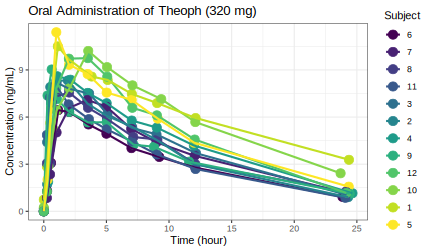
\includegraphics[width=1\linewidth]{pharmapk_files/figure-latex/ggtheoph-1} 

}

\caption{Concentration-time curves of oral administration of Theoph (N = 12)}\label{fig:ggtheoph}
\end{figure}

\hypertarget{loading}{%
\section{자료 불러오기}\label{loading}}

\texttt{read.csv()} 함수를 사용해서 자료를 불러 옵니다.
엑셀 파일을 사용하는 경우 \texttt{readxl} 패키지를 설치한 후에 \texttt{read\_excel()} 함수를 사용해서 불러올 수 있습니다.
다만 이 경우 \texttt{tibble} 형태로 자료가 변형되므로 \texttt{as.data.frame()}을 사용해서 데이타프레임으로 변형해주어야 합니다.

\hypertarget{ruxc744-uxc774uxc6a9uxd55c-uxbe44uxad6cuxd68duxbd84uxc11d-uxc2e4uxc81c-1}{%
\section{R을 이용한 비구획분석 실제 1}\label{ruxc744-uxc774uxc6a9uxd55c-uxbe44uxad6cuxd68duxbd84uxc11d-uxc2e4uxc81c-1}}

\hypertarget{tblnca-uxc804uxccb4-uxb300uxc0c1uxc790-uxbe44uxad6cuxd68d-uxbd84uxc11d}{%
\subsection{tblNCA(): 전체 대상자 비구획 분석}\label{tblnca-uxc804uxccb4-uxb300uxc0c1uxc790-uxbe44uxad6cuxd68d-uxbd84uxc11d}}

가장 많이 쓰는 함수 입니다!
NonCompart 패키지의 핵심적인 기능입니다.
아래의 코드를 R의 콘솔창에 넣어보세요.
테오필린 경구 투여시의 비구획 분석입니다.

결과는 \texttt{data.frame} 형태인데 너무 길기 때문에 핵심적인 일부 파라메터 (C\textsubscript{max}, T\textsubscript{max}, AUC\textsubscript{last})만 표시할 수도 있습니다.

\begin{verbatim}
##    Subject  CMAX TMAX AUCLST
## 1        1 10.50 1.12 148.92
## 2        2  8.33 1.92  91.53
## 3        3  8.20 1.02  99.29
## 4        4  8.60 1.07 106.80
## 5        5 11.40 1.00 121.29
## 6        6  6.44 1.15  73.78
## 7        7  7.09 3.48  90.75
## 8        8  7.56 2.02  88.56
## 9        9  9.03 0.63  86.33
## 10      10 10.21 3.55 138.37
## 11      11  8.00 0.98  80.09
## 12      12  9.75 3.52 119.98
\end{verbatim}

인도메타신 정맥 투여시의 비구획 분석입니다.
함수인자 \texttt{adm}을 infusion으로 바꾼 것을 볼 수 있고 \texttt{dur}가 추가된 것을 볼 수 있습니다.

역시 핵심적인 일부 파라메터 (C\textsubscript{max}, T\textsubscript{max}, AUC\textsubscript{last})만 표시할 수도 있습니다.

\begin{verbatim}
##   Subject CMAX TMAX AUCLST
## 1       1 1.50 0.25  1.741
## 2       2 2.03 0.25  2.933
## 3       3 2.72 0.25  2.934
## 4       4 1.85 0.25  2.478
## 5       5 2.05 0.25  1.954
## 6       6 2.31 0.25  2.873
\end{verbatim}

\hypertarget{snca}{%
\subsection{sNCA()}\label{snca}}

한명의 대상자에 대해 비구획 분석을 시행합니다.

\begin{verbatim}
##         b0       CMAX      CMAXD       TMAX       TLAG 
##    2.36879   10.50000    0.03281    1.12000    0.00000 
##       CLST      CLSTP       TLST     LAMZHL       LAMZ 
##    3.28000    3.28015   24.37000   14.30438    0.04846 
##     LAMZLL     LAMZUL    LAMZNPT     CORRXY         R2 
##    9.05000   24.37000    3.00000   -1.00000    1.00000 
##      R2ADJ     AUCLST     AUCALL     AUCIFO    AUCIFOD 
##    1.00000  148.92305  148.92305  216.61193    0.67691 
##     AUCIFP    AUCIFPD     AUCPEO     AUCPEP    AUMCLST 
##  216.61496    0.67692   31.24892   31.24988 1459.07110 
##    AUMCIFO    AUMCIFP    AUMCPEO    AUMCPEP       VZFO 
## 4505.53482 4505.67086   67.61603   67.61701   30.48675 
##       VZFP       CLFO       CLFP   MRTEVLST   MRTEVIFO 
##   30.48632    1.47730    1.47728    9.79748   20.80003 
##   MRTEVIFP 
##   20.80037 
## attr(,"units")
##  [1] ""          "mg/L"      "mg/L/mg"   "h"        
##  [5] "h"         "mg/L"      "mg/L"      "h"        
##  [9] "h"         "/h"        "h"         "h"        
## [13] ""          ""          ""          ""         
## [17] "h*mg/L"    "h*mg/L"    "h*mg/L"    "h*mg/L/mg"
## [21] "h*mg/L"    "h*mg/L/mg" "%"         "%"        
## [25] "h2*mg/L"   "h2*mg/L"   "h2*mg/L"   "%"        
## [29] "%"         "L"         "L"         "L/h"      
## [33] "L/h"       "h"         "h"         "h"        
## attr(,"UsedPoints")
## [1]  9 10 11
\end{verbatim}

이때의 그림은 다음과 같습니다. (Figure \ref{fig:ggtheophindi})

\begin{figure}

{\centering 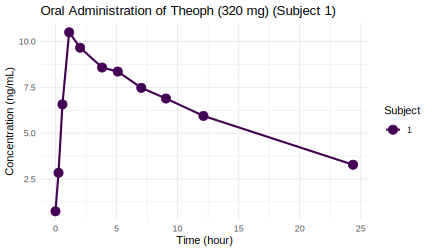
\includegraphics[width=1\linewidth]{pharmapk_files/figure-latex/ggtheophindi-1} 

}

\caption{Individual concentration-time curves of oral administration of Theoph (Subject 1)}\label{fig:ggtheophindi}
\end{figure}

\hypertarget{uxae30uxc220uxd1b5uxacc4-descriptive-statistics}{%
\subsection{기술통계 (Descriptive statistics)}\label{uxae30uxc220uxd1b5uxacc4-descriptive-statistics}}

R에서는 필요에 따라서 자신만의 함수를 만들 수도 있습니다.
아래를 실행하면 \texttt{desc\_tblNCA()} 함수를 사용하여 기술통계량을 쉽게 구할 수 있습니다. (Table \ref{tab:theodesc} and \ref{tab:indodesc})

\begin{table}

\caption{\label{tab:theodesc}Descriptive statistics of selected PK parameters of Theoph oral administration}
\centering
\begin{tabular}[t]{lrrrrrr}
\toprule
  & n & mean & sd & median & min & max\\
\midrule
Subject* & 12 & 6.500 & 3.606 & 6.500 & 1.00 & 12.00\\
CMAX & 12 & 8.759 & 1.473 & 8.465 & 6.44 & 11.40\\
TMAX & 12 & 1.788 & 1.112 & 1.135 & 0.63 & 3.55\\
AUCLST & 12 & 103.807 & 23.645 & 95.407 & 73.78 & 148.92\\
\bottomrule
\end{tabular}
\end{table}

\begin{table}

\caption{\label{tab:indodesc}Descriptive statistics of selected PK parameters of Indometh IV infusion}
\centering
\begin{tabular}[t]{lrrrrrr}
\toprule
  & n & mean & sd & median & min & max\\
\midrule
Subject* & 6 & 3.500 & 1.8708 & 3.500 & 1.000 & 6.000\\
CMAX & 6 & 2.077 & 0.4136 & 2.040 & 1.500 & 2.720\\
TMAX & 6 & 0.250 & 0.0000 & 0.250 & 0.250 & 0.250\\
AUCLST & 6 & 2.485 & 0.5267 & 2.675 & 1.741 & 2.934\\
\bottomrule
\end{tabular}
\end{table}

\hypertarget{ruxc744-uxc774uxc6a9uxd55c-uxbe44uxad6cuxd68duxbd84uxc11d-uxc2e4uxc81c-2}{%
\section{R을 이용한 비구획분석 실제 2}\label{ruxc744-uxc774uxc6a9uxd55c-uxbe44uxad6cuxd68duxbd84uxc11d-uxc2e4uxc81c-2}}

웹브라우저를 통해 간단히 비구획분석을 할 수 있는 앱을 개발하였습니다.

\begin{itemize}
\tightlist
\item
  Han, S. (2017) pkrshiny: Noncompartmental Analysis using pkr R package Shiny application. URL: \url{https://asan.shinyapps.io/pkrshiny}
\end{itemize}

그 외 약동학과 관련된 몇가지 shiny 앱도 참고하세요.

\begin{itemize}
\tightlist
\item
  Han, S. (2017) Pharmacokinetic Simulation of one-compartment Models. URL: \url{https://asan.shinyapps.io/pk1c/}
\item
  Han, S. (2017) caff: Monte Carlo Simulation of Caffeine Shiny application. URL: \url{https://asan.shinyapps.io/caff}
\item
  Han, S. (2016) vtdm: Vancomycin TDM Shiny application. URL: \url{https://asan.shinyapps.io/vtdm}
\end{itemize}

\hypertarget{uxbe44uxad6cuxd68duxbd84uxc11d-uxbcf4uxace0uxc11c}{%
\section{비구획분석 보고서}\label{uxbe44uxad6cuxd68duxbd84uxc11d-uxbcf4uxace0uxc11c}}

ncar은 보고서를 만드는 패키지입니다. 현재 설정된 working directory에 결과 파일이 생성됩니다.

\hypertarget{txtnca}{%
\subsection{txtNCA()}\label{txtnca}}

txtNCA()를 통해서 다음 결과를 얻을 수 있습니다.

파일로 저장하려면 다음을 입력합니다.

\begin{verbatim}
## Error in file(con, "w"): 커넥션을 열 수 없습니다
\end{verbatim}

\hypertarget{pdfnca}{%
\subsection{pdfNCA()}\label{pdfnca}}

pdfNCA()로 pdf로 결과를 볼 수 있습니다. (Figure \ref{fig:pdfnca-output})

\begin{verbatim}
## Error in pdf(FileName, paper = Paper, width = 8.5, height = 11, family = FontFamily, : 파일 'Output-ncar/pdfNCA-Theoph.pdf'를 열 수 없습니다
\end{verbatim}

\begin{verbatim}
## Error in knitr::include_graphics(c("Output-ncar/pdfNCA-Theoph-01.png", : Cannot find the file(s): "Output-ncar/pdfNCA-Theoph-01.png"; "Output-ncar/pdfNCA-Theoph-02.png"
\end{verbatim}

\hypertarget{rtfnca}{%
\subsection{rtfNCA()}\label{rtfnca}}

마이크로소프트 워드에서 편집가능한 rtf파일을 만듭니다.

\hypertarget{pkrplotpk}{%
\subsection{pkr::plotPK()}\label{pkrplotpk}}

비구획분석에 대한 다양한 시각화는 여러 유용한 정보를 제공해 줍니다.
이를 가능하게 해 주는 \texttt{pkr} 패키지(\protect\hyperlink{ref-R-pkr}{\textbf{R-pkr?}})에 대해서 자세히 알아보겠습니다.

\begin{verbatim}
## pdf 
##   2
\end{verbatim}

\hypertarget{pkr-manual}{%
\subsection{pkr 사용법}\label{pkr-manual}}

\texttt{pkr} 함수의 가장 핵심적인 기능은 \texttt{plotPK()} 함수에 있고 이 함수의 인자는 다음과 같습니다.

\begin{verbatim}
## function (concData, id, Time, conc, unitTime = "hr", unitConc = "ng/mL", 
##     trt = "", fit = "Linear", dose = 0, adm = "Extravascular", 
##     dur = 0, outdir = "Output") 
## NULL
\end{verbatim}

\texttt{Theoph} 자료의 그림을 그리는 명령어를 실행해 보겠습니다.

\begin{verbatim}
## pdf 
##   2
\end{verbatim}

조금 기다린 후 \texttt{Output} 폴더를 확인해 보면 세개의 그림 파일이 생성된 것을 알 수 있습니다.

\begin{itemize}
\tightlist
\item
  ./Output/PK Profile Linear Scale for Theoph.tiff
\item
  ./Output/PK Profile Log 10 Scale for Theoph.tiff
\item
  ./Output/PK Profile with CI for Theoph.tiff
\end{itemize}

\begin{verbatim}
## Error in knitr::include_graphics("Output/PK_Profile_Linear_Scale_for_Theoph.png"): Cannot find the file(s): "Output/PK_Profile_Linear_Scale_for_Theoph.png"
\end{verbatim}

\begin{verbatim}
## Error in knitr::include_graphics("Output/PK_Profile_Log_10_Scale_for_Theoph.png"): Cannot find the file(s): "Output/PK_Profile_Log_10_Scale_for_Theoph.png"
\end{verbatim}

\begin{verbatim}
## Error in knitr::include_graphics("Output/PK_Profile_with_CI_for_Theoph.png"): Cannot find the file(s): "Output/PK_Profile_with_CI_for_Theoph.png"
\end{verbatim}

또한 개개인 별로 여러개의 그림이 담긴 두개의 PDF 파일이 생성되었습니다.

\begin{itemize}
\tightlist
\item
  ./Output/Individual PK Linear Scale for Theoph.pdf
\item
  ./Output/Individual PK Log 10 Scale for Theoph.pdf
\end{itemize}

\begin{verbatim}
## Error in knitr::include_graphics("Output/Individual_PK_Linear_Scale_for_Theoph.png"): Cannot find the file(s): "Output/Individual_PK_Linear_Scale_for_Theoph.png"
\end{verbatim}

\begin{verbatim}
## Error in knitr::include_graphics("Output/Individual_PK_Log_10_Scale_for_Theoph.png"): Cannot find the file(s): "Output/Individual_PK_Log_10_Scale_for_Theoph.png"
\end{verbatim}

\hypertarget{parameters}{%
\section{파라메터의 의미}\label{parameters}}

비구획분석 시 여러 파라메터가 나오며 약어로 표현하는 경우가 많습니다. 또한 소프트웨어마다 약어가 상이하기 때문에 자주 그 의미를 찾아볼 필요가 있습니다. 콘솔창에 다음을 입력합니다.

ncar::RptCfg의 일부를 첨부합니다. (Table \ref{tab:rptcfg}) \texttt{PPTESTCD}는 NonCompart 패키지에서 출력하는 파라메터 이름이며, CDISC SDTM PPTESTCD (Parameter Short Name)\footnote{다음과 같이 CDISC note에 표시되어 있습니다. `Short name of the pharmacokinetic parameter. It can be used as a column name when converting a dataset from a vertical to a horizontal format. The value in PPTESTCD cannot be longer than 8 characters, nor can it start with a number (e.g., ``1TEST''). PPTESTCD cannot contain characters other than letters, numbers, or underscores. Examples: ``AUCALL,'' ``TMAX,'' ``CMAX.''\,' \url{https://wiki.cdisc.org/pages/viewpage.action?pageId=42309513}}와 같은 값입니다. \texttt{WNL} 열은 Certara Phoenix WinNonLin에서 구한 파라메터 이름입니다.

\begin{longtable}[t]{ll}
\caption{\label{tab:rptcfg}Description of NonCompart parameters}\\
\toprule
PPTESTCD & Description (WNL)\\
\midrule
b0 & Intercept (b0)\\
TLAG & Time Until First Nonzero Conc (Tlag)\\
MRTEVLST & MRT Extravasc to Last Nonzero Conc (MRTlast)\\
MRTEVIFO & MRT Extravasc Infinity Obs (MRTINF\_obs)\\
MRTEVIFP & MRT Extravasc Infinity Pred (MRTINF\_pred)\\
\addlinespace
VZFO & Vz Obs by F (Vz\_F\_obs)\\
VZFP & Vz Pred by F (Vz\_F\_pred)\\
CLFO & Total CL Obs by F (Cl\_F\_obs)\\
CLFP & Total CL Pred by F (Cl\_F\_pred)\\
C0 & Initial Conc (C0)\\
\addlinespace
AUCPBEO & AUC \%Back Extrapolation Obs (AUC\_.Back\_Ext\_obs)\\
AUCPBEP & AUC \%Back Extrapolation Pred (AUC\_.Back\_Ext\_pred)\\
CMAX & Max Conc (Cmax)\\
CMAXD & Max Conc Norm by Dose (Cmax\_D)\\
TMAX & Time of CMAX (Tmax)\\
\addlinespace
CLST & Last Nonzero Conc (Clast)\\
TLST & Time of Last Nonzero Conc (Tlast)\\
CLSTP & Last Nonzero Conc Pred (Clast\_pred)\\
LAMZHL & Half-Life Lambda z (HL\_Lambda\_z)\\
LAMZ & Lambda z (Lambda\_z)\\
\addlinespace
LAMZLL & Lambda z Lower Limit (Lambda\_z\_lower)\\
LAMZUL & Lambda z Upper Limit (Lambda\_z\_upper)\\
LAMZNPT & Number of Points for Lambda z (No\_points\_lambda\_z)\\
CORRXY & Correlation Between TimeX and Log ConcY (Corr\_XY)\\
R2 & R Squared (Rsq)\\
\addlinespace
R2ADJ & R Squared Adjusted (Rsq\_adjusted)\\
AUCLST & AUC to Last Nonzero Conc (AUClast)\\
AUCALL & AUC All (AUCall)\\
AUCIFO & AUC Infinity Obs (AUCINF\_obs)\\
AUCIFOD & AUC Infinity Obs Norm by Dose (AUCINF\_D\_obs)\\
\addlinespace
AUCPEO & AUC \%Extrapolation Obs (AUC\_.Extrap\_obs)\\
AUCIFP & AUC Infinity Pred (AUCINF\_pred)\\
AUCIFPD & AUC Infinity Pred Norm by Dose (AUCINF\_D\_pred)\\
AUCPEP & AUC \%Extrapolation Pred (AUC\_.Extrap\_pred)\\
AUMCLST & AUMC to Last Nonzero Conc (AUMClast)\\
\addlinespace
AUMCIFO & AUMC Infinity Obs (AUMCINF\_obs)\\
AUMCPEO & AUMC \%Extrapolation Obs (AUMC\_.Extrap\_obs)\\
AUMCIFP & AUMC Infinity Pred (AUMCINF\_pred)\\
AUMCPEP & AUMC \% Extrapolation Pred (AUMC\_.Extrap\_pred)\\
MRTIVLST & MRT Intravasc to Last Nonzero Conc (MRTlast)\\
\addlinespace
MRTIVIFO & MRT Intravasc Infinity Obs (MRTINF\_obs)\\
MRTIVIFP & MRT Intravasc Infinity Pred (MRTINF\_pred)\\
VZO & Vz Obs (Vz\_obs)\\
VZP & Vz Pred (Vz\_pred)\\
CLO & Total CL Obs (Cl\_obs)\\
\addlinespace
CLP & Total CL Pred (Cl\_pred)\\
VSSO & Vol Dist Steady State Obs (Vss\_obs)\\
VSSP & Vol Dist Steady State Pred (Vss\_pred)\\
\bottomrule
\end{longtable}

\hypertarget{ca-principle}{%
\chapter{구획 분석의 이론}\label{ca-principle}}

\Large\hfill

임동석
\normalsize

\begin{center}\rule{0.5\linewidth}{0.5pt}\end{center}

\hypertarget{uxad6cuxd68duxbd84uxc11duxc758-uxac1cuxb150}{%
\section{구획분석의 개념}\label{uxad6cuxd68duxbd84uxc11duxc758-uxac1cuxb150}}

\hypertarget{uxad6cuxd68duxbaa8uxb378uxc774-uxd544uxc694uxd55c-uxc774uxc720}{%
\section{구획모델이 필요한 이유}\label{uxad6cuxd68duxbaa8uxb378uxc774-uxd544uxc694uxd55c-uxc774uxc720}}

\hypertarget{uxad6cuxd68duxbaa8uxb378-uxd30cuxb77cuxbbf8uxd130uxb4e4uxc758-uxc758uxbbf8uxc640-uxc8fcuxc758uxc810}{%
\section{구획모델 파라미터들의 의미와 주의점}\label{uxad6cuxd68duxbaa8uxb378-uxd30cuxb77cuxbbf8uxd130uxb4e4uxc758-uxc758uxbbf8uxc640-uxc8fcuxc758uxc810}}

\hypertarget{uxb9fauxc74cuxb9d0-2}{%
\section{맺음말}\label{uxb9fauxc74cuxb9d0-2}}

\hypertarget{ca-analysis}{%
\chapter{구획분석의 자료해석}\label{ca-analysis}}

\Large\hfill

한성필
\normalsize

\begin{center}\rule{0.5\linewidth}{0.5pt}\end{center}

\hypertarget{uxc0c1uxc6a9-uxc18cuxd504uxd2b8uxc6e8uxc5b4uxb97c-uxc774uxc6a9uxd55c-uxad6cuxd68d-uxbd84uxc11d-uxac1cuxb860}{%
\section{상용 소프트웨어를 이용한 구획 분석 개론}\label{uxc0c1uxc6a9-uxc18cuxd504uxd2b8uxc6e8uxc5b4uxb97c-uxc774uxc6a9uxd55c-uxad6cuxd68d-uxbd84uxc11d-uxac1cuxb860}}

\hypertarget{uxad6cuxd68duxbd84uxc11duxc5d0-uxd65cuxc6a9uxd560-uxc218-uxc788uxb294-r-package-uxc18cuxac1c}{%
\section{구획분석에 활용할 수 있는 R package 소개}\label{uxad6cuxd68duxbd84uxc11duxc5d0-uxd65cuxc6a9uxd560-uxc218-uxc788uxb294-r-package-uxc18cuxac1c}}

\hypertarget{uxad6cuxd68duxbd84uxc11duxc744-uxc704uxd55c-uxb370uxc774uxd130uxc14buxc758-uxc791uxc131}{%
\section{구획분석을 위한 데이터셋의 작성}\label{uxad6cuxd68duxbd84uxc11duxc744-uxc704uxd55c-uxb370uxc774uxd130uxc14buxc758-uxc791uxc131}}

\hypertarget{uxad6cuxd68duxbaa8uxb378uxc744-uxc774uxc6a9uxd55c-uxc815uxb9e5uxc8fcuxc0ac-uxd6c4-uxc57duxb3d9uxd559-uxc790uxb8cc-uxbd84uxc11d-1}{%
\section{1구획모델을 이용한 정맥주사 후 약동학 자료 분석 1}\label{uxad6cuxd68duxbaa8uxb378uxc744-uxc774uxc6a9uxd55c-uxc815uxb9e5uxc8fcuxc0ac-uxd6c4-uxc57duxb3d9uxd559-uxc790uxb8cc-uxbd84uxc11d-1}}

\hypertarget{uxad6cuxd68duxbaa8uxb378uxc744-uxc774uxc6a9uxd55c-uxc815uxb9e5uxc8fcuxc0ac-uxd6c4-uxc57duxb3d9uxd559-uxc790uxb8cc-uxbd84uxc11d-2}{%
\section{1구획모델을 이용한 정맥주사 후 약동학 자료 분석 2}\label{uxad6cuxd68duxbaa8uxb378uxc744-uxc774uxc6a9uxd55c-uxc815uxb9e5uxc8fcuxc0ac-uxd6c4-uxc57duxb3d9uxd559-uxc790uxb8cc-uxbd84uxc11d-2}}

\hypertarget{uxad6cuxd68duxbaa8uxb378uxc744-uxc774uxc6a9uxd55c-uxacbduxad6cuxd22cuxc5ec-uxd6c4-uxc57duxb3d9uxd559-uxc790uxb8cc-uxbd84uxc11d-1}{%
\section{1구획모델을 이용한 경구투여 후 약동학 자료 분석 1}\label{uxad6cuxd68duxbaa8uxb378uxc744-uxc774uxc6a9uxd55c-uxacbduxad6cuxd22cuxc5ec-uxd6c4-uxc57duxb3d9uxd559-uxc790uxb8cc-uxbd84uxc11d-1}}

\hypertarget{uxad6cuxd68duxbaa8uxb378uxc744-uxc774uxc6a9uxd55c-uxacbduxad6cuxd22cuxc5ec-uxd6c4-uxc57duxb3d9uxd559-uxc790uxb8cc-uxbd84uxc11d-2}{%
\section{1구획모델을 이용한 경구투여 후 약동학 자료 분석 2}\label{uxad6cuxd68duxbaa8uxb378uxc744-uxc774uxc6a9uxd55c-uxacbduxad6cuxd22cuxc5ec-uxd6c4-uxc57duxb3d9uxd559-uxc790uxb8cc-uxbd84uxc11d-2}}

\hypertarget{uxad6cuxd68duxbaa8uxb378uxc744-uxc774uxc6a9uxd55c-uxc57duxb3d9uxd559-uxc790uxb8cc-uxbd84uxc11d}{%
\section{2구획모델을 이용한 약동학 자료 분석}\label{uxad6cuxd68duxbaa8uxb378uxc744-uxc774uxc6a9uxd55c-uxc57duxb3d9uxd559-uxc790uxb8cc-uxbd84uxc11d}}

\hypertarget{uxb9fauxc74cuxb9d0-3}{%
\section{맺음말}\label{uxb9fauxc74cuxb9d0-3}}

\printindex

\end{document}
